\section{Our Approach}\label{sec:approach}

Figure~\ref{fig:overview} provides an overview of the whole pipeline that we employ to create an effective mathematics-aware language model. Now the diagram is focused on the \textsc{Qwen2.5-1.5B} checkpoint, and this process can generalize to any decoder-only transformer of similar size. The pipeline consists of four successive stages, see below.\\

\textbf{(1) Data curation and pre-processing.}
We start by collecting various mathematics corpora: open-source proof repositories, competition problems, and questions which are selected from educational websites, question-answer pairs (QAPs). After removing duplicates, the raw pool has 3M candidate sentences. A lightweight heuristic filter discards non-mathematical text and malformed \LaTeX\ text, resulting in over 260 K high-quality examples. The token for each sample is then tokenized using the original \texttt{qwen.tiktoken} tokenizer and trimmed or zero-padded to a maximum length of 512 tokens to be compatible with the model’s context window.\\

\textbf{(2) Preparing the model.}
The vanilla Hugging Face checkpoint contains \texttt{nn.Linear}, \texttt{nn.LayerNorm}, and \texttt{RMSNorm} modules. We write a one-for-one replacement that exchanges these layers for their highest quality NVIDIA Transformer Engine (TE) counterpart, thus enabling native FP8 execution on Hopper GPUs without modifying the weight tensors. A configuration file also switches on grouped-query attention (GQA) and rotary positional embeddings so that the fine-tuned model follows the most recent Qwen2 architectural specifications.\\

\textbf{(3) Precision-Aware Fine-Tuning.}
We continue training for three epochs with a global batch size of 26 × 4 = 104 sequences, which we achieve using the gradient-accumulation loop from Section~\ref{sec:gradacc}. We adopt the hybrid FP8 recipe (E4M3 for weight/activations, E5M2 for gradients) explained in Section~\ref{sec:precision_recipes}. The learning-rate dynamics are controlled by an AdamW optimizer with \(\beta_1=0.9\), \(\beta_2=0.95\), and a 50 step cosine warm-up. Checkpoints are saved every 1,000 optimization steps along with parameter-efficient \texttt{wandb} logs of perplexity and token-level accuracy.\\

\textbf{(4) Serving/receiving and judging.}
At the end, the highest scoring FP8 checkpoint is transferred to the \texttt{vLLM} inference engine, which flows tokens with paged attention and speculative decoding. On a H100 NVL, during inference, we obtain a throughput of 102.5 tokens/s at a latency of 11.8 ms ± 0:2 ms using only 1:70 GiB of device memory. Functional correctness is tested against GSM8K and MATH dev sets, the fine-tuned model outperforms FP32 baseline in avg-exact-k by 4.6\% abs-pnt. The released final artifacts, i.e., the model weight, tokenizer, and evaluation scripts are licensed to be open to downstream research community.

    
\begin{figure}[h]
    \centering
    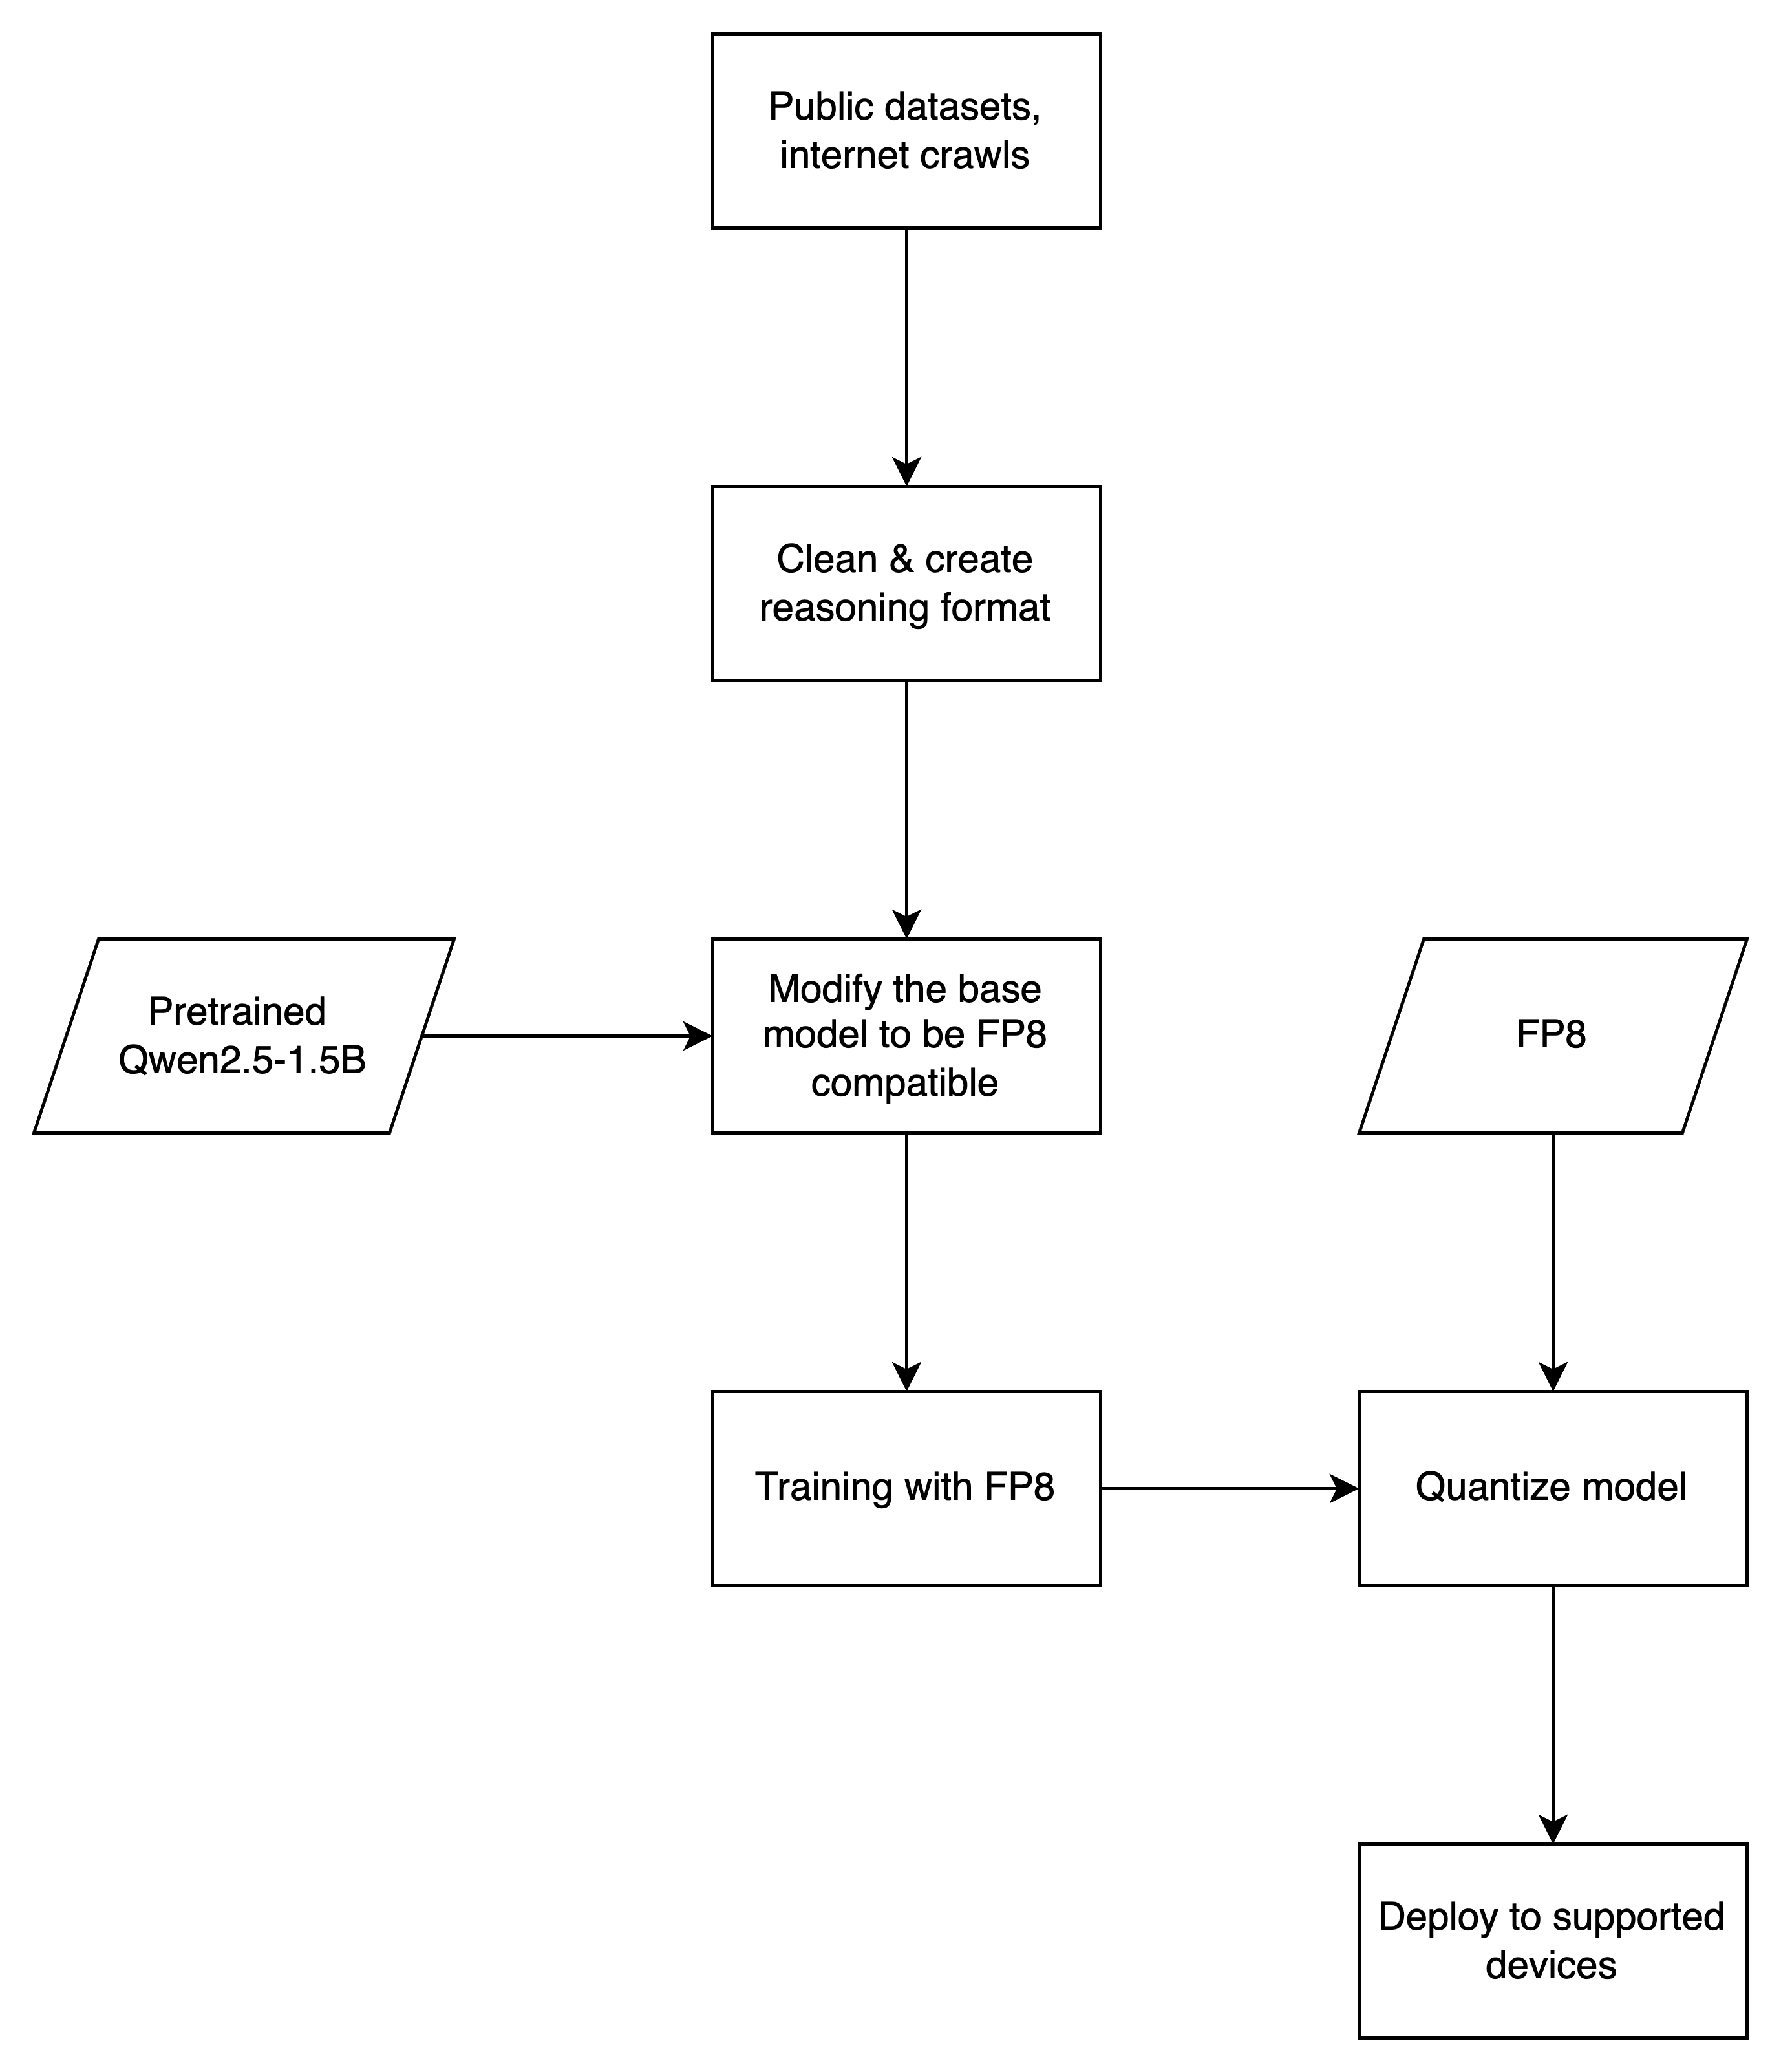
\includegraphics[width=0.75\linewidth]{figures/c1/overview.drawio.png}
    \caption{End-to-end pipeline for data construction, precision convert, fine-tune, and deploy the \textsc{Qwen2.5-1.5B} model.}
    \label{fig:overview}
\end{figure}
